\def\V{\text{\sc Vrai}\,}
\def\F{\text{\sc Faux}\,}
\def\ite{\text{\sc ite}\,}
%-------------------------------------------------------------------------------
%-------------------------------------------------------------------------------
\chapter{Bidons}
%-------------------------------------------------------------------------------
%-------------------------------------------------------------------------------
\thispagestyle{empty}
%-------------------------------------------------------------------------------
%-------------------------------------------------------------------------------
Dupont et Dupond se sont perdus dans le désert et leur jeep est en panne. 

\begin{center}
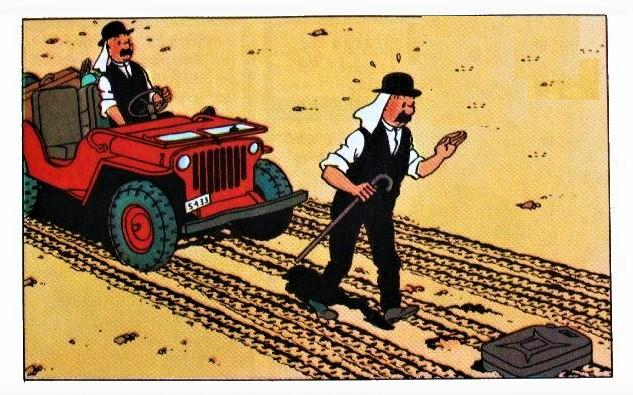
\includegraphics[width=0.8\textwidth]{dupond_t}
\end{center}


Il leur reste un bidon de huit litres d'eau, ainsi que deux bidons vides dont les capacités respectives sont de cinq et trois litres. 

Dupont pense qu'il faut marcher vers le nord, mais Dupond penche pour le sud. 

Ils décident donc de se séparer, mais ils veulent partager l'eau équitablement.

Nous allons les aider !

Associons aux trois bidons un triplet $(a, b, c)$ qui indique le nombre de litres d'eau que chacun contient ; au départ on a $(a, b, c) = (8, 0, 0)$. Une opération élémentaire consiste à verser de l'eau d'un bidon x dans un bidon y jusqu'à ce que y soit plein ou que x soit vide. 
Par exemple, on peut passer de la situation initiale $(8, 0, 0)$ à la situation $(3, 5, 0)$ ou à la situation $(5, 0, 3)$ selon que l'on décide de remplir le deuxième ou le troisième bidon.

On note \type{init} la situation initiale $(8, 0, 0)$.

\medskip

Derrière ce problème de partage se profile donc un graphe : ses sommets sont les valeurs possibles de
$(a, b, c)$ compatibles avec la capacité initiale. Ce graphe est orienté : un arc mène de $(a, b, c)$ à $(a', b', c')$ si l'on peut passer de la première situation à la deuxième au moyen d'une opération élémentaire. Nous noterons ceci $(a, b, c) \rightarrow (a', b', c')$.
%-------------------------------------------------------------------------------
\newpage
%-------------------------------------------------------------------------------
\begin{Exercise}
{\it Combien ce graphe compte-t-il de sommets ?}
\end{Exercise}
%-------------------------------------------------------------------------------
\begin{Answer}

Un état est déterminé par la capacité des petits bidons, $b$ et $c$, car alors le gros bidon a une capacité de $8 - b - c$. $b\in \{0,1,2,3,4,5\}$ et $c\in \{0,1,2,3\}$ donc il y a 24 états.
\end{Answer}
%-------------------------------------------------------------------------------
%-------------------------------------------------------------------------------
\begin{Exercise}
{\it Résoudre le problème à la main.}
\end{Exercise}
%-------------------------------------------------------------------------------
\begin{Answer}

Voici une solution, l'autre est obtenue en changeant le deuxième état en $(5, 0, 3)$ :

$(8,0,0) \rightarrow (3,5,0) \rightarrow (3,2,3) \rightarrow (6,2,0) \rightarrow (6,0,2) \rightarrow (1,5,2) \rightarrow (1,4,3) \rightarrow (4,4,0)$
\end{Answer}
%-------------------------------------------------------------------------------
%-------------------------------------------------------------------------------
\begin{Exercise}
{\it Montrez que , pour tout état $t$ distinct de \type{init} avec 8 litres au total, 

alors soit $t \rightarrow  \type{init}$ 
soit il existe un état $t'$ tel que $t \rightarrow t'$ et $t' \rightarrow \type{init}$.}
\end{Exercise}
%-------------------------------------------------------------------------------
\begin{Answer}
On vide les deux petits bidons dans le grand.
\end{Answer}
%-------------------------------------------------------------------------------
%-------------------------------------------------------------------------------
%-------------------------------------------------------------------------------
\section{Généralisation}
%-------------------------------------------------------------------------------
%-------------------------------------------------------------------------------
%-------------------------------------------------------------------------------

On définit les types 
\begin{lstlisting}

type bidon = {maxi : int ; actu : int};;
type etat = bidon array;;
\end{lstlisting}

Le champ \type{maxi} permet de traiter le problème avec des bidons de capacités quelconques.
%-------------------------------------------------------------------------------
%-------------------------------------------------------------------------------
\begin{Exercise}
{\it Écrire une fonction \type{opElem (x,y)} qui effectue  l'opération élémentaire consistant à déverser le bidon \type{x} dans le bidon \type{y}. }
\begin{lstlisting}
opElem : bidon * bidon -> bidon * bidon
\end{lstlisting}
\end{Exercise}
%-------------------------------------------------------------------------------
\begin{Answer}
\begin{lstlisting}
let opElem (x, y) = 
  let q = min (y.maxi - y.actu) x.actu in 
  ({maxi = x.maxi ; actu = x.actu - q}, 
   {maxi = y.maxi ; actu = y.actu + q});;
\end{lstlisting}
\end{Answer}
%-------------------------------------------------------------------------------
%-------------------------------------------------------------------------------
\begin{Exercise}
{\it Écrire  une fonction \type{voisins s} qui construit la liste des états $t$ tels que $s \rightarrow t$ avec $s\ne t$.}
\begin{lstlisting}
voisins : etat -> etat list
\end{lstlisting}
\end{Exercise}
%-------------------------------------------------------------------------------
\begin{Answer}
\begin{lstlisting}
let voisins e = 
   let n = Array.length e in
   let a = ref [] in
   for i = 0 to (n-1) do
      for j = 0 to (n-1) do
         if i <> j
         then begin
            let (x, y) = opElem (e.(i), e.(j)) in
            if (x, y) <> (e.(i), e.(j))
            then begin
               let e1 = Array.copy e in
               e1.(i) <- x;
               e1.(j) <- y;
               a := e1 :: !a end end done done;
   !a;;
\end{lstlisting}
\end{Answer}
%-------------------------------------------------------------------------------
%-------------------------------------------------------------------------------
On dit qu'il existe un chemin de $s$ à $t$ s'il existe une suite $(t_k )_{0\le k \le n}$ de sommets telle que :
$t_0 = s$, $t_n = t$ et $t_{k-1}\rightarrow t_k$ pour tout tel que $1\le k\le n$.
%-------------------------------------------------------------------------------
%-------------------------------------------------------------------------------
\begin{Exercise}\it 

Pour un état $e$ donné, déterminer les états $f$ tels qu'il existe un chemin de $e$ vers $f$.

On pourra utiliser une liste de sommets vus ; on cherchera un sommet dans cette miste avec la fonction 
\begin{lstlisting}
List.mem : 'a -> 'a liste -> bool
\end{lstlisting}
\end{Exercise}
%-------------------------------------------------------------------------------
\begin{Answer}
On maintient les états à voir dans une liste et on y ajoute les voisins au fur et à mesure qu'on les calcule.
\begin{lstlisting}
let accessibles e = 
  let rec lire vus a_voir =
    match a_voir with
    |[] -> vus
    |f::reste ->  if List.mem f vus
                  then lire vus reste
                  else let plus = voisins f in
                       lire (f::vus) (reste@plus) in
  lire [] [e];;
\end{lstlisting}
On peut remplacer \type{reste\@plus} par \type{plus\@reste}.
\newpage
\end{Answer}
%-------------------------------------------------------------------------------
%-------------------------------------------------------------------------------
\begin{Exercise}
{\it Écrire une fonction qui donne un chemin entre $e$ et $e$ quand celui-ci existe.}
\end{Exercise}
%-------------------------------------------------------------------------------
\begin{Answer}
Il faut modifier la recherche de composante en insérant le chemin.
\begin{lstlisting}
let joli e =
   let n = Array.length e in
   let t = Array.make n 0 in
   for i = 0 to (n-1) do
      t.(i) <- e.(i).actu done;
   t;;
  
let chemin e f = 
   let rec faire vus a_voir =
      match a_voir with
      |[] -> failwith "Il n'y a pas de chemin"
      |(chm, s)::reste when List.mem s vus -> faire vus reste
      |(chm, s)::reste when s = f -> List.rev ((joli s) :: chm)
      |(chm, s)::reste -> let chm' = (joli s) :: chm in 
                          let plus x = (chm', x) in
                          let suite = List.map plus (voisins s) in
                          faire (s::vus) (reste@suite) 
   in faire [] [e];;
\end{lstlisting}
\end{Answer}
%-------------------------------------------------------------------------------
%-------------------------------------------------------------------------------



